\documentclass[12pt]{article}
\usepackage[top=2cm,bottom=3cm,left=3cm,right=3cm]{geometry} %define borders

\usepackage{url}
\usepackage{paralist}
\usepackage{xcolor}
\usepackage{multicol}
\usepackage{graphicx}
\usepackage[bookmarksnumbered,bookmarksopen,colorlinks,urlcolor=gray,linkcolor=blue,citecolor=blue]{hyperref}



\begin{document}

\title{Knowledge Hosting}
\author{Behrooz bozorgchamy}
\date{\today}
\maketitle{}
\begin{abstract}
    Knowledge graphs (KGs) use a graph-based structure to show the representation of connections between entities and nodes. Graph-based structure introduces unique challenges for storage and managing it. This paper explores the primary challenges in hosting KGs and evaluates three major paradigms: relational databases, document stores, and graph databases, with a focus on RDF triplestores. We analyze the advantages and disadvantages of each approach with a real-world example, the German Tourism Knowledge Graph (GTKG). Our findings show that graph databases, particularly RDF triplestores, best address KG-specific requirements, offering flexible schemas, native reasoning, and efficient querying. This study provides insights for practitioners and researchers in selecting appropriate hosting solutions for large-scale KGs.

    Keywords: Knowledge Graphs, Hosting Paradigms, RDF Triplestores, Relational Databases, Document Stores, Graph Databases
\end{abstract}

\section{Introduction}
Knowledge graphs are built by nodes (entities) and edges (relationships), which enable the representation of complex, interconnected data. Many applications use knowledge graphs as a base, such as search engines, recommendation systems, and data integration. Nevertheless, storing and hosting it has significant challenges related to scale, data models, and operational demands (CRUD). This paper synthesizes key concepts from recent advancements in KG hosting, focusing on paradigms that balance efficiency, flexibility, and reasoning capabilities.

We start by highlighting the challenges in KG hosting. Section 3 reviews hosting paradigms: relational databases, document stores, graph databases, and RDF triplestores. A case study on the German Tourism Knowledge Graph (GTKG) illustrates practical implementation (Section 5). Finally, we conclude with implications and future directions.
\begin{figure}
    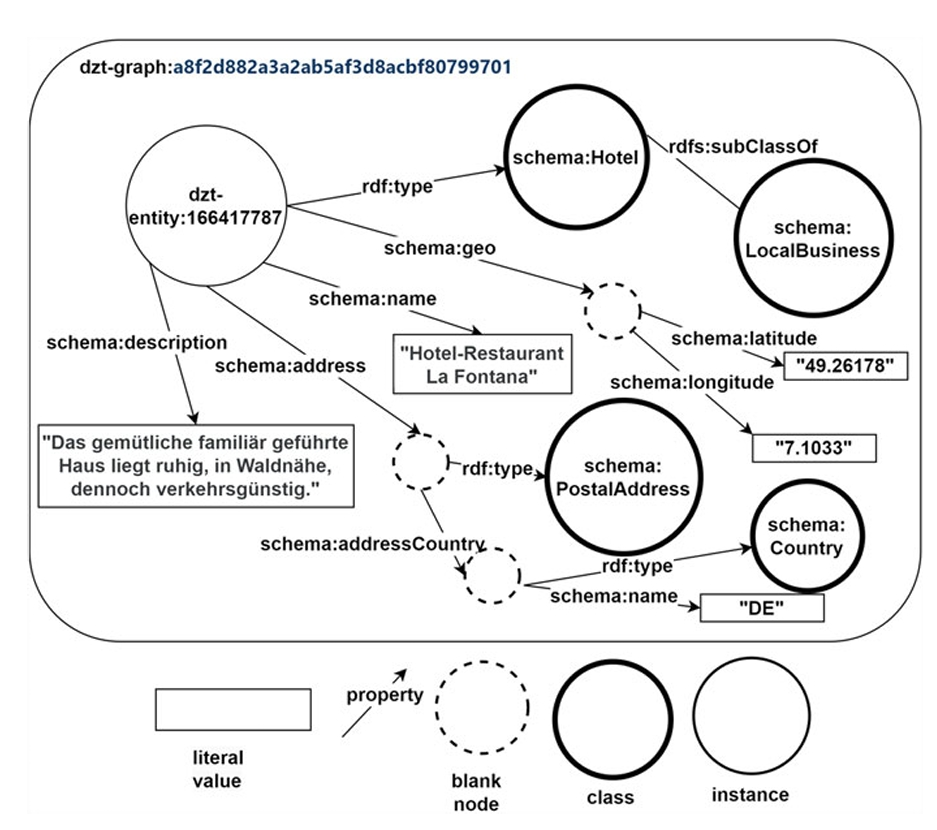
\includegraphics[width=\linewidth]{imgs/gtkg-example.jpeg}
    \label{fig:gtkg-example}
    \caption{An excerpt from the German Tourism Knowledge Graph}
\end{figure}
\section{Challenges in Hosting Knowledge Graphs}
Hosting KGs needs to address several interrelated challenges.
\begin{itemize}
    \item \textbf{Size}: KGs can have billions of facts and need scalable storage and efficient retrieval mechanisms to handle massive datasets without performance issues.
    \item \textbf{Data model}: KGs adopt a graph structure (semantic networks), where vertices represent concepts and edges denote relations. Representing this in a non-native structure leads to inefficiencies, such as excessive joins or data redundancy.
    \item \textbf{Heterogeneity}: KGs by nature have a flexible schema, and they often integrate data from diverse sources with varying schemas, which the hosting solution should support.
    \item \textbf{Velocity}: KGs change rapidly by inference, integration of new sources, or updates. Systems have control over high-frequency changes while maintaining consistency.
    \item \textbf{Point of view}: Every application has its own requirements, such as contextual constraints or inference rules. Ideal hosts should support this.
    \item \textbf{Deployment}: KGs must be accessible via multiple interfaces (e.g., APIs, query languages) and formats to serve diverse applications, from web services to analytical tools.

\end{itemize}
These challenges underscore the need for paradigms that natively align with graph semantics while providing robustness and adaptability.
\section{Knowledge Hosting Paradigms}
KGs are logically graph-based; however, they can be hosted on various database paradigms. We evaluate relational databases, document stores, and graph databases, highlighting their pros and cons relative to the challenges.
\subsection{Relational Databases}
Relational databases, based on Codd's model (1970), are the most famous database paradigm. Relational databases store data in tables with tuples and relations, queried via SQL. Operations like Join, Projection, and Selection facilitate data manipulation. You can see an example of it in Fig. \ref{fig:rd-example}. However, they don’t support RDF Schema (RDFS) naively, which is an issue of this paradigm and must be handled by applications. Moreover, representing class and property hierarchies often demands numerous auxiliary tables and complex joins. As a result, the application must explicitly embed the semantics into its code.

Ultimately, for various reasons, application logic must explicitly encode the semantics of modeling languages like RDFS, which undermines the declarative nature and reusability of knowledge graphs. Below, we will discuss four primary approaches for storing knowledge graphs in relational databases (Ben Mahria et al., 2021).

\begin{figure}
    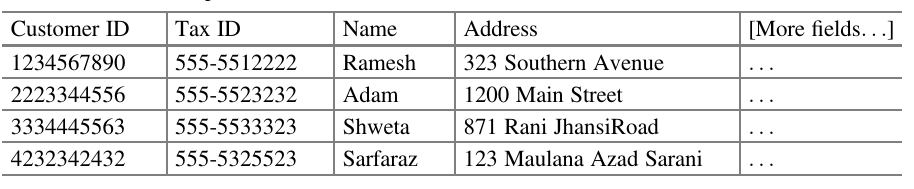
\includegraphics[width=\linewidth]{imgs/rd-example.jpeg}
    \label{fig:rd-example}
    \caption{An example of Relational database}
\end{figure}

\subsubsection{Statement Tables}
Single table with columns for subject, predicate, and object. Simple and most forward but
prone to inefficient self-joins for large graphs. Because this approach result is a big table
which has all information. Moreover, Statement Table approach has another drawback,
the data is not normalized So, value replications can happen. The example of it is Fig. \ref{fig:Statement-Tables-example}

\begin{figure}
    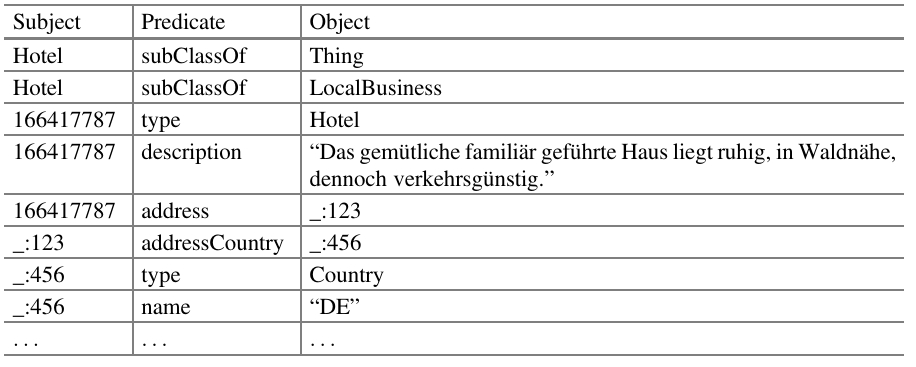
\includegraphics[width=\linewidth]{imgs/Statement table.jpeg}
    \label{fig:Statement-Tables-example}
    \caption{An example of Statement Tables }
\end{figure}

\subsubsection{Class-centric table}
The class-centric approach uses one table per type, storing all property values in a single table. Properties may appear in multiple tables if shared by classes. Table 19.6 partially represents the knowledge graph from Fig. \ref{fig:gtkg-example}, with each class as a table and properties as columns. Properties without values in the graph become columns with NULL values, leading to sparse tables. A separate table (Table 19.6a) stores class hierarchies, enabling queries like “list all LocalBusiness instances” by joining with the Hotel table (Table 19.6b).

Each type uses a separate table for its properties, making modeling intuitive. However, this approach has drawbacks. Adding new properties or classes requires schema recompilation. For instance, creating an event type instance involves adding a table and columns in the relational database schema. Additionally, normalization struggles with multivalued properties, causing tuple repetition. For example, multiple hotel descriptions require additional tuples with repeated values for other columns.
\subsubsection{Property-centric}
Property-centric tables use one table per property, each with subject and object columns. This supports multivalued properties but requires subject duplication. Table 19.7 partially shows the property-centric storage of the knowledge graph in Fig. \ref{fig:gtkg-example}, focusing on hotel instance properties for brevity. Like the class-centric approach, it has drawbacks: adding new properties requires creating new tables and schema recompilation, and retrieving an instance’s properties involves joining many tables.
\subsubsection{Virtual RDF graphs}
The last one, virtual RDF graphs, provides an ontology-based access layer over relational databases, transforming SPARQL queries into SQL for execution, with results mapped back to SPARQL. Popular for converting relational databases to knowledge graphs, the process (Fig. 19.2) involves rewriting SPARQL queries per the ontology, unfolding them using schema-to-ontology mappings, and executing the resulting SQL. Optimizations include offline ontology compilation, exploiting data constraints to simplify queries, and cost-based query planning. Ontop10 (Xiao et al. 2020), an Apache 2-licensed framework, supports R2RML, SPARQL 1.1 subsets, and OWL 2 QL reasoning via query rewriting.
\begin{multicols}{2}
    Advantages:
    \begin{itemize}
        \item No RDBMS preprocessing needed.
        \item Enables ontology-based access via mappings and query rewriting.
        \item Cost-effective for building knowledge graphs from relational databases.
        \item Integrates well with standard software environments.
    \end{itemize}
    \columnbreak
    Drawbacks:
    \begin{itemize}
        \item Query rewriting and unfolding can be error-prone.
        \item Schema querying is challenging due to the relational model.
        \item Limited querying and reasoning capabilities.
    \end{itemize}
\end{multicols}
\subsection{Document Stores}
Document stores manage data as nested key-value pairs (e.g., JSON documents) in collections, without enforced schemas, which means each document in a collection can have a different schema. This paradigm suits big data and streaming due to scalability.

The document stores model for knowledge graphs is schemaless, enabling looser consistency checks and supporting heterogeneity and velocity. Instances can have varied metadata and multiple property values, avoiding relational database issues like null values or duplications. Many implementations natively support JSON documents, providing O(1) access for retrieving instances in JSON-LD format, where each instance is a document. Which makes it a good option.

The document model paradigm can host KGs in two ways: nested objects and document references.
\subsubsection{Nested objects}
The nested object approach stores all instance data in a single document, simplifying access. However, updating nested objects across multiple documents is challenging and typically managed by application logic or middleware. Figure 19.3 depicts the knowledge graph from Fig. \ref{fig:gtkg-example} as nested objects, with blank nodes represented by nested objects lacking an id field.
\subsubsection{Document references}
The document reference approach organizes documents into cohesive collections, storing references instead of nested objects. This simplifies updates compared to nested objects but requires application-level join operations, blurring the line between document stores and relational databases. Figure 19.4 partially represents the knowledge graph from Fig. \ref{fig:gtkg-example}, with separate collections for Hotel and PostalAddress instances. A hotel's address property, a blank node in the graph, uses an internally unique ID (e.g., \_:123) from the PostalAddress collection.

Many document store implementations can host knowledge graphs. For example, HexaDB implements an RDF triplestore using RocksDB as its key-value backend, with indexing optimizations. AllegroGraph offers a document store backend alongside its graph-based model.

\subsection{Graph Databases}
Graph databases represent data and schemas as graphs, with data manipulation via graph transformations. Many support flexible schemas, and some offer data integrity features like constraints and referential integrity (Angles and Gutierrez 2008). Nodes (entities) and edges (relationships) can have varying metadata, defining their capabilities. For knowledge graphs, we focus on two types: property graphs and RDF triplestores.
\subsubsection{Property graphs}
Property graphs model, the most popular approach, relationships between entities using nodes and edges.
Nodes represent entities, can store key-value properties, and are labeled to indicate their role or type.

Edges connect nodes, are directional, are labeled to show relationship type, and can also hold properties.

There’s no formal standard for property graphs; development is industry-led. A popular implementation is Neo4J, which uses the Cypher query language. For example, you can query all hotels named Hotel-Restaurant La Fontana using Cypher.
\begin{verbatim}
MATCH (h:Hotel {name: 'Hotel-Restaurant La Fontana'}) RETURN h
\end{verbatim}
The main disadvantage of this way is the lack of standardized technologies for querying and native reasoning capabilities. RDF triplestores tried to address these issues.
\subsubsection{RDF triplestores}
RDF graph databases, or triplestores, store triples per the RDF model, optimized for this structure. They support RDFS and OWL2 reasoning with built-in reasoners and use SPARQL 1.1 for querying, often with APIs. Many use relational or document store backends, but recent implementations natively support RDF graphs (Karvinen et al. 2019). Triplestores offer flexible schemas, blending schema and data for querying, and follow W3C standards (RDF, RDFS, OWL, SPARQL), aiding vendor migration and tooling. A survey lists 135 triplestore implementations, some scaling to trillions of triples (Ali et al. 2021). Unlike property graphs, which support statements about relationships but lack native reasoning, RDF triplestores provide reasoning but struggle with statements about statements. Extensions like Named Graphs and RDF-Star add metadata for context like temporal validity or provenance. Efforts to bridge property graphs and RDF include Neo4j's Neosemantics plugin, supporting RDF technologies, and AnzoGraph, which handles both models. Standardization for graph databases continues.
\section{Real-world Application: German Tourism Knowledge Graph (GTKG) in GraphDB}
The German Tourism Knowledge Graph is hosted in an RDF triplestore called GraphDB from Ontotext. GraphDB provides all major functionalities needed for hosting KGs, such as storing, querying, visualizing, and reasoning of RDF graphs.

In this section, we will demonstrate what these functionalities look like with the help of our running example presented in the German Tourism Knowledge Graph (GTKG).

The GTKG, hosted in GraphDB Enterprise, contains over 13M statements integrating tourism data from 16 German states, including events, tours, and POIs. Data is organized in named graphs, each representing a state’s tourism marketing organization, e.g., Saarland’s data in \verb|dzt-graph:a8f2d882a3a2ab5af3d8acbf80799701|, enabling provenance tracking and licensing access control. RDF graphs can be loaded via GUI, API, or SPARQL INSERT queries. Figure 19.5 shows a tabular view of the graph from Fig. \ref{fig:gtkg-example}, with statements about \verb|dzt-entity:-1664177870| organized in the Saarland named graph. This graph’s IRI is used to assert properties like dataset creation dates (December 2021, February 2022) and publisher via schema.org and PROV-O terminology, as shown in Fig. 19.6.

GraphDB offers a graphical interface and API for running SPARQL 1.1 queries. By default, queries target the union of all named graphs in a repository unless a named graph is specified using FROM NAMED or GRAPH keywords, which scopes the triple patterns. Figure 19.7 shows the interface executing a query to retrieve 1000 triples from the Saarland named graph, using the GRAPH keyword to bind the graph’s IRI and filter by the publisher’s name property.

GraphDB offers three main visualizations for RDF datasets: class hierarchy, class relationships, and visual graph. The class hierarchy uses a Venn diagram view, with circles representing classes and their subclasses, sized by instance count. Figure 19.8 shows schema:Thing as a top class in the GTKG, aiding visual debugging for class errors. Class relationship visualization highlights links between class instances, e.g., ~520K schema:geo links from schema:Place to schema:GeoCoordinates (Fig. 19.9), showing key types by connectedness. The visual graph displays incoming and outgoing edges for a resource’s IRI or SPARQL-selected subgraph (Fig. \ref{fig:gtkg-example}0), initially showing 1-hop connections, with configurable, interactive node expansion.

GraphDB’s reasoner infers new facts from existing ones using W3C-recommended entailment rules in a forward-chaining approach. Its materialization strategy applies inference rules at load time, increasing loading time but speeding up queries. Supported reasoning profiles include RDF(S), RDFS-Plus, and OWL2 profiles (Horst, DL, QL, RL), each suited for different use cases. RDFS-Plus, used by the GTKG, supports subsumption, inverse, and transitive property reasoning (Allemang et al. 2020). OWL-Horst, a non-W3C profile, optimizes performance for large datasets. GraphDB uses two virtual named graphs: explicit (loaded triples) and implicit (inferred triples). Queries can target explicit statements only or both, e.g., querying “All Local businesses” in Fig. \ref{fig:gtkg-example} returns no results with explicit statements but retrieves schema:Hotel instances with both due to subsumption reasoning.
\section{Conclusion}
KG hosting demands paradigms that accommodate graph semantics, scale, and dynamism. Relational databases offer integrity but rigidity; document stores provide flexibility for annotations but weak connectivity; graph databases, especially RDF triplestores, emerge as optimal, balancing all challenges with native reasoning and standards.

Future work could be enhanced reasoning for emerging KG applications. The GTKG case underscores practical viability, guiding deployments in tourism and beyond.
\end{document}
